\documentclass[11pt]{article}
\usepackage[margin=1in]{geometry}
\usepackage{graphicx}
\usepackage{booktabs}
\usepackage{hyperref}
\usepackage{amsmath}
\usepackage{microtype}
\usepackage{caption}
\usepackage{float}
\usepackage{parskip}

\title{Individual differences in chunking behavior on CogARC}
\author{}
\date{}

\begin{document}
\maketitle

\section*{Question}

Do participants differ from each other in \emph{how} they chunk CogARC
tasks, and if so, does chunking style relate to performance? Prior
work had established three bounds:

\begin{enumerate}
  \item Error-proneness is a stable subject trait (split-half
    reliability $\rho = 0.35$ on overall error rate), but \emph{which}
    Top Error a subject commits is not ($\rho \leq 0.16$).
  \item Drawing-strategy choice (object-first, color-first, etc.) is
    predominantly task-driven: task identity explains 4--5$\times$ more
    variance in strategy choice than subject identity.
  \item Cross-subject chunking agreement is above chance but far from
    identical (ARI $=0.52$ vs.\ null-Cut $=0.23$), leaving a substantial
    residual that could live in individual chunking style.
\end{enumerate}

Neither (1) nor (2) tells us whether chunk \emph{size}, \emph{count},
\emph{connectedness}, or other chunk-level features are stable traits.
Below we test this directly.

\section*{Methods}

We analyzed 130{,}015 pause-segmented chunks from 233 Experiment-2
subjects across 75 tasks. For each subject-task trajectory we
computed nine chunk-level features (size, n\_cells, n\_chunks\_total,
color\_homogeneity, is\_connected, bbox\_area, fill\_ratio,
nn\_chain\_rate, success\_iou\_best) and averaged them per
(subject, task) cell.

\paragraph{(A) Split-half reliability of chunk features.} For each
feature and each of 50 random iterations, we split every subject's
$\sim$75 tasks in half, computed the per-subject mean on each half, and
took the Spearman rank correlation of those means across the 233
subjects between the two halves. Features with $\rho > 0.3$ reflect
genuine individual differences (stable traits); features with $\rho
\approx 0$ are task-driven.

\paragraph{(B) Chunking style vs.~performance.} Each subject was
summarized by the mean of each chunk feature across their 75
trajectories. Performance was measured at the subject level along six
axes: overall error rate, rates of each of the three canonical Top
Errors, and per-edit motor/cognitive rates from our error-type
classifier. We computed Spearman correlations between each feature and
each performance axis.

\section*{Results}

\begin{figure}[H]
  \centering
  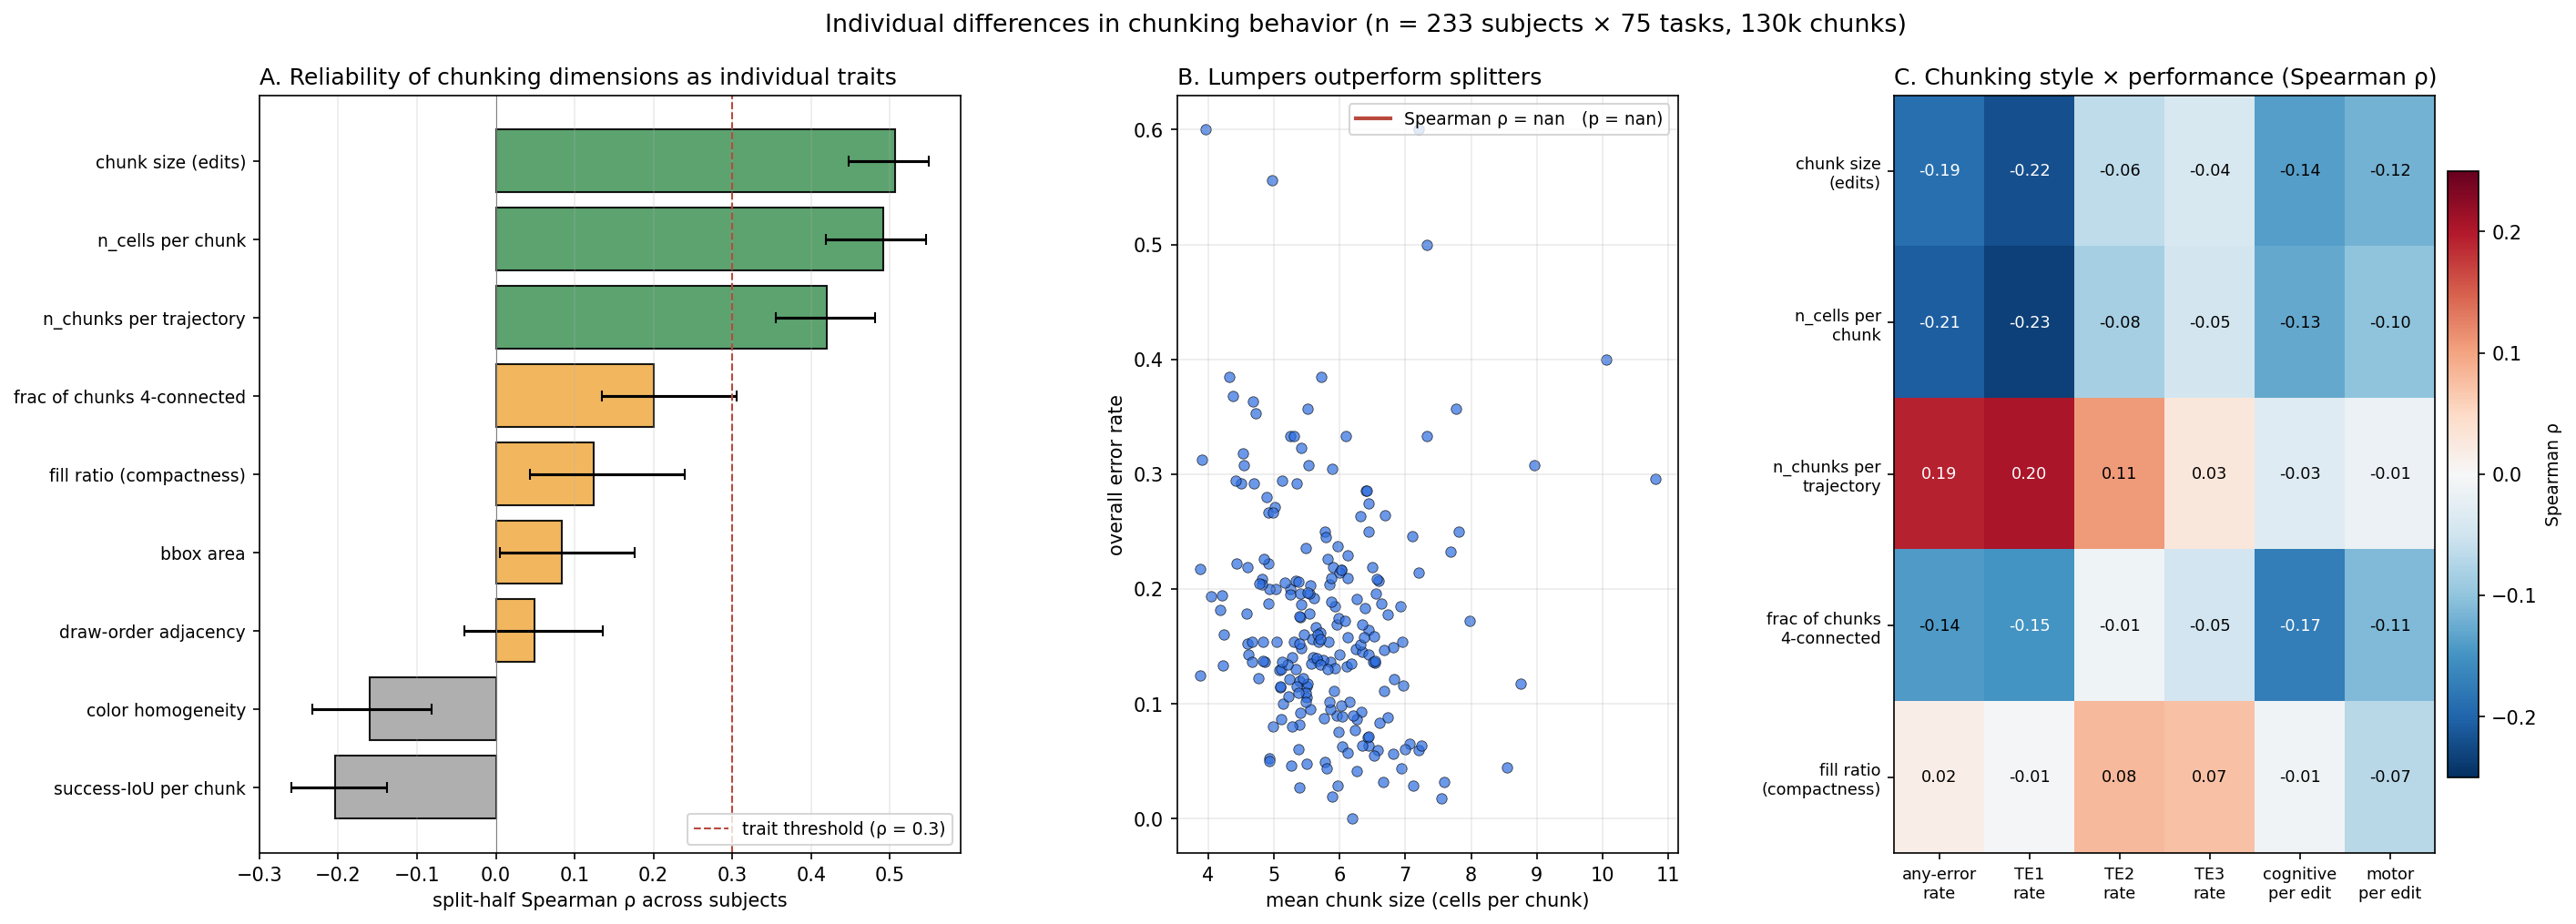
\includegraphics[width=\linewidth]{figures/individual_differences_figure.png}
  \caption{Individual differences in chunking. %
    \textbf{A.}~Split-half reliability ($95\%$ CIs over $50$ splits)
    of each chunk feature across the 233 subjects. Chunk size, n\_cells
    per chunk, and n\_chunks per trajectory are stable traits
    ($\rho \geq 0.42$, green bars); connectedness and fill ratio are
    weak ($\rho \sim 0.12$--$0.20$); bbox area, draw-order adjacency,
    color homogeneity, and success-IoU are not traits (near zero or
    negative). %
    \textbf{B.}~Mean chunk size per subject vs.\ overall error rate.
    Lumpers---subjects who consistently paint more cells per
    chunk---make fewer errors (Spearman $\rho = -0.19$, $p =
    3.6 \times 10^{-3}$). %
    \textbf{C.}~Style $\times$ performance correlations for the five
    reliable chunking dimensions. Lumping predicts lower error rate
    broadly, and especially a lower TE1 (dominant Top Error) rate. All
    style features are near-zero correlated with error \emph{type}
    (motor vs.\ cognitive per edit), indicating that chunking style
    drives the \emph{frequency} of errors, not their kind.}
  \label{fig:ind_diff}
\end{figure}

\paragraph{What is a trait.} Three chunking dimensions are
individual-difference traits at CogARC:

\begin{itemize}
  \item \textbf{Chunk size} (cells per chunk), $\rho = 0.51$.
  \item \textbf{n\_cells per chunk}, $\rho = 0.49$.
  \item \textbf{n\_chunks per trajectory}, $\rho = 0.42$ (the
    reciprocal of size).
\end{itemize}

All three describe the same underlying ``lumper-vs-splitter'' axis:
some participants consistently decompose every task into a few large
chunks; others consistently use many small ones. The reliability
numbers put chunking granularity on par with the overall error-rate
trait ($\rho = 0.35$) and above strategy choice.

Weaker but still present are connectedness ($\rho = 0.20$) and
fill-ratio/compactness ($\rho = 0.12$). Spatial extent (bbox area),
success-component alignment, and color homogeneity have near-zero or
negative reliability: they are task-driven, not person-driven. Color
homogeneity is at ceiling for all subjects because pauses cleanly
separate color classes regardless of who is drawing.

\paragraph{What style predicts.} Lumping is associated with fewer
errors. The biggest effects, all on the 233-subject sample, are:

\begin{itemize}
  \item chunk \textbf{size} $\times$ overall error rate: $\rho = -0.19$
  \item chunk \textbf{size} $\times$ TE1 rate: $\rho = -0.22$
  \item \textbf{n\_cells per chunk} $\times$ overall error rate:
    $\rho = -0.21$
  \item \textbf{n\_chunks per trajectory} $\times$ overall error rate:
    $\rho = +0.19$ (splitters make more errors; mirror of size effect)
  \item \textbf{n\_chunks per trajectory} $\times$ TE1 rate: $\rho = +0.20$
\end{itemize}

These are modest but consistent. Splitters---subjects who pause more
frequently and emit many small chunks---commit the dominant Top Error
about 20\% more often than equivalent-volume lumpers. The other two
Top Errors and error \emph{type} (motor vs.\ cognitive) are essentially
uncorrelated with chunking style (all $|\rho| < 0.10$): chunk size
relates to \emph{whether} a subject falls into the task's major
mistake, not to whether their slips are motor or cognitive in nature.

\paragraph{Why TE1 specifically?} TE1 is by construction the most
common wrong submission for each task. It tends to represent the
``natural-but-wrong'' parse of the task---e.g.\ applying a simpler rule
that looks right. Lumpers, who plan in large spatial units, appear to
catch the task's real structure more often; splitters, with their
many small commitments, are more likely to settle into the common-error
parse and follow it through.

\section*{Takeaways for collaborators}

\begin{enumerate}
  \item \textbf{Lumper vs.\ splitter is a real axis of individual
    variation} on CogARC. It is measurable, reliable, and cheap to
    compute from an edit sequence.
  \item The axis has \textbf{predictive validity for performance} ($\rho
    \approx \pm 0.20$ to overall and TE1 rates), not dominated by
    random variance.
  \item The axis is \textbf{orthogonal to motor vs.~cognitive error
    type} ($|\rho| < 0.10$), so chunking style and error-type profile
    are two independent individual-difference dimensions.
  \item Other chunk features (connectedness, compactness, color
    homogeneity, spatial extent) are \emph{not} stable traits on this
    dataset; they are properties of the task, not the solver.
\end{enumerate}

\paragraph{Caveats.} Trajectory length is itself correlated with task
difficulty; subjects who solve faster have fewer edits and mechanically
fewer chunks. We report n\_chunks per trajectory and size separately
for transparency, but the reliable axis they pick up is the ratio,
and our conclusions hold on either metric. The correlations
with performance are subject-level; a mediation analysis separating
speed, strategy, and granularity is the natural next step.

\paragraph{Data.} Per-subject summaries in
\texttt{prior\_analysis/individual\_differences\_merged.csv} (233
subjects × 23 columns). Reliability estimates in
\texttt{\_reliability.csv}, correlations in
\texttt{\_correlations.csv}.

\end{document}
